\documentclass[a4paper, english]{scrartcl}

\usepackage[english]{babel}
\usepackage{tabularx}
\usepackage{graphicx}
\usepackage{booktabs}
\usepackage{microtype}
% TODO Fix title below
\usepackage[pdftitle = {TODO TITLE HERE}, colorlinks = true, urlcolor = blue, linkcolor = blue, citecolor = blue]{hyperref}

% TODO Fix title here
\title{Optical Character Recognition}
\subtitle{Subtitle here \ldots}
% TODO Add names here
\author{Irvin,~Duane \\ \texttt{duane@student.chalmers.se}
  \and Karlsson,~Pontus \\ \texttt{ponkarls@student.chalmers.se}
  \and Holm,~Jesper \\ \texttt{~holmje@student.chalmers.se}
  \and Subramanian,~Aditya \\ \texttt{email@student.chalmers.se}
}
\date{DATE HERE, 2017}

\begin{document}

\clearpage\maketitle
\thispagestyle{empty}

\pagebreak

\setcounter{page}{1}
\hypersetup{linkcolor=black}
\tableofcontents

\pagebreak

\section{Introduction}
\subsection{Background}
Literacy, the ability to read, is a core skill in the modern, information age
that we live in. Unfortunately, many people around the world suffer from
illiteracy due to reasons such as visual impairment, learning disabilities or
a lack of opportunity. Providing a solution to this problem could prove
fruitful in incorporating these people into our society. However, such a
solution to the illiteracy problem could prove costly both from a fiscal and
resource perspective. Optical Character Recognition technology could be the
key to solving this problem at a low opportunity cost.
\subsection{Purpose}
In cooperation with Cybercom, a software is to be developed which recognises
characters from an image and outputs it as an audio recording.
\subsection{Vision}
The vision of the final product is to have a smartphone application which
works on both Android and Apple’s iOS. The product should support both video
feeds and static images as input and both text and audio outputs. In addition
to character recognition, word recognition and the ability to self-correct in
case of false recognition should be implemented. The recognition rate of all
the above features should match the industry standard of 95\%.

\subsection{Scope}
Due to time constraints word recognition and word correction features will not
 be implemented. The application will run on a laptop and not be ported to
 smartphones. The input will be in the form of still images and not a video
 feed. The industry standard 95\% recognition rate is also unachievable with
 the current time constraints and is instead adjusted to a 60\% recognition
 rate.

Features below are denoted with RF for required features and OF for optional
features.
  \noindent\begin{tabularx}{\linewidth}{X p{0.75\linewidth}}
  \toprule
    \textbf{Feature} & \textbf{Description} \\
  \midrule
  RF-1 &
    From an image, recognize characters with an accuracy of at least 60\%. \\
  RF-2 &
    Turn text into English speech output. \\
  RF-3 &
    User interface that implements RF-1 and RF-2. \\
  OF-1 &
    Add functionality and improve performance to make the product compatible
    with mobile devices. \textit{TBD} \\
  OF-2 &
    Use dictionary for correction of recognized words. \textit{TBD} \\
  OF-3 &
    Improve RF-1 to 90\% recognition rate. \\
  \bottomrule
  \end{tabularx}

\section{Method}
\textit{TBD}

\subsection{Testing}
\textit{TBD}

\section{Technical Background}
\textit{TBD}

\section{Implementation}

\subsection{UML/Modules}
\textit{TBD}
\begin{figure}[h!]
  \centering
  % TODO Fix label
  \caption{\textit{TBD}}\label{fig:ex1a}
  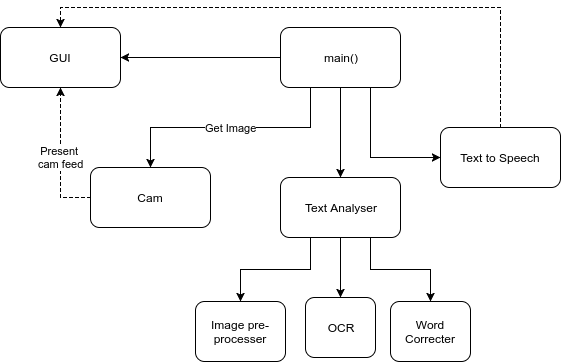
\includegraphics[width=1.0\textwidth]{res/UML1}
\end{figure}

\subsection{Optical Character Recognition}
\textit{TBD}

\subsection{GUI}
\textit{TBD}

\subsection{Text-To-Speech}
\textit{TBD}

\subsection{Tests}
\textit{TBD}

\section{Result}
\textit{TBD}

\section{Discussion}
\textit{TBD}

\pagebreak
% Ask me how to properly insert references // Duane
\bibliography{references}
\bibliographystyle{ieeetr}

\end{document}
